 \pagebreak[4]
 \hspace*{1cm}
 \pagebreak[4]
 \hspace*{1cm}
 \pagebreak[4]

\chapter{TỔNG QUAN}
\ifpdf
    \graphicspath{{Chapter1/Chapter1Figs/PNG/}{Chapter1/Chapter1Figs/PDF/}{Chapter1/Chapter1Figs/}}
\else
    \graphicspath{{Chapter1/Chapter1Figs/EPS/}{Chapter1/Chapter1Figs/}}
\fi

\markboth{\MakeUppercase{\thechapter. My Third Chapter }}{\thechapter. TỔNG QUAN}
  
\section{Đặt vấn đề}
	Ngày nay, công nghệ phát triển không ngừng và ngày càng ảnh hưởng sâu rộng vào đời sống xã hội, dần dần trở thành một phần không thể thiếu trong xã hội loài người. Trong sự phát triển đó thì công nghệ thông tin đống một vai trò chủ chốt không thể thiếu. Với sự những tiến bộ vượt bậc trong lĩnh vực trí tuệ nhân tạo (Artificial Intelligence) mà điển hình và thị giác máy tính (computer vision). Những công nghệ này đã và đang giúp con người giải quyết được những bài toán thực tế trong đời sống và làm cho xã hội ngày ngày càng văn minh hiện đại hơn.\par
	Với sự phát triển nhanh chóng của khoa học kỹ thuật và công nghệ, hệ thống thiết bị thu phát hình ảnh như camera giám sát ngày càng hiện đại và phổ biến với chất lượng ngày càng cao cùng chi phí triển khai ở mức thấp. Các hệ thống này thường được sử dụng để theo giỏi và đánh giá tình hình anh ninh trật tự ở các địa điểm công cộng (công viện, trường học, quảng trường, nhà ga, sân bay,...), các cơ quan trọng yếu (tòa nhà, cơ quan công quyền, các khu vực an ninh quốc phòng). Hay những hệ thống giám sát giao thông theo giỏi tình hình tắc nghẽn tại các điểm nóng giao thông hay tình hình phương tiện giao thông thời gian cao điểm. Với đối tượng giám sát là con người, một trong những hành vi của con người cần được ưu tiên giám sát đó là hành vi tụ tập đông người (đám đông). \par
\begin{figure}[ht]
  			\begin{center}
    				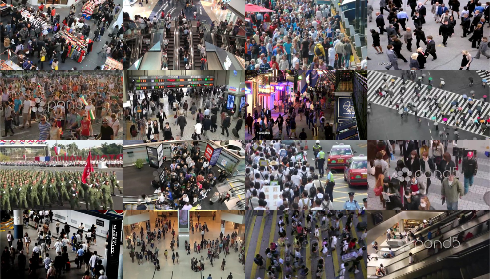
\includegraphics[scale=0.7]{damdong} 
    				\caption{Dữ liệu hình giám sát đám đông (nguồn: Internet)} 
    				\label{damdong}
  			\end{center}
\end{figure}	
	 Vào ngày 24 tháng 7 năm 2010, lễ hội âm nhạc Love Parade \footnote{$https://en.wikipedia.org/wiki/Love\_Parade\_disaster$} được tổ chức tại Đức ở một ga vận tải củ với sức chứa tối đa là 250,000 người, nhưng thực tế đã có hơn nửa triệu khác du lịch đến tham gia lễ hội, dẫn đến xảy ra một vụ thảm họa về đám đông. Vụ việc này đã cướp đi sinh mạng của 21 người và ít nhất 500 người bị thương. Một vụ tương tự cũng xảy ra tại Ấn Độ, vào ngày 14 tháng 1 năm 2011, là ngày Makara Jyothi\footnote{$https://en.wikipedia.org/wiki/Love\_Parade\_disaster$}. Một cuộc hành hương thường niên hàng năm diễn ra ở gần đền thờ Sabarimala cũng đã cướp đi sinh mạng của 106 người hành hương và làm bị thương gần 100 người. Những sự việc trên có thể sẽ không phải xảy ra nếu chúng ta có một hệ thống giám sát và ước lượng đượng mật độ đám đông, từ đó đưa ra những cảnh báo về khả năng xảy ra những thảm họa như trên. Không những thế  việc có thể ước lượng hay tính toán được mật độ của đám đông có thể áp dụng trong rất nhiều bối cảnh như những cuộc biểu tình, những sự kiện chính trị, những sân vận động bóng đá, thông tin cho lĩnh vực quảng cáo, hay cảnh báo và đưa ra chiến lược giải quyết các vấn đề ùn tắc với đối tượng là các phương tiện giao thông. \par
\begin{figure}%
\centering
\subfigure[]{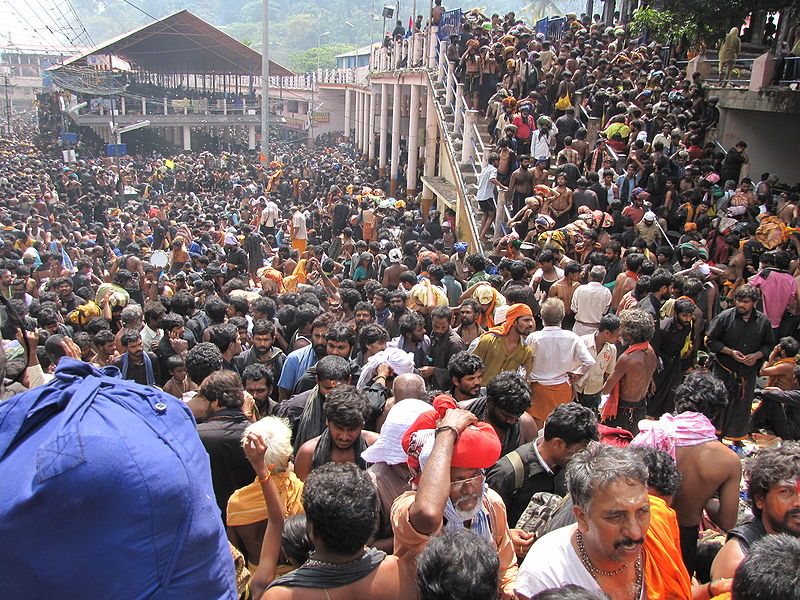
\includegraphics[width=.45\linewidth]{ab}}\qquad
\subfigure[]{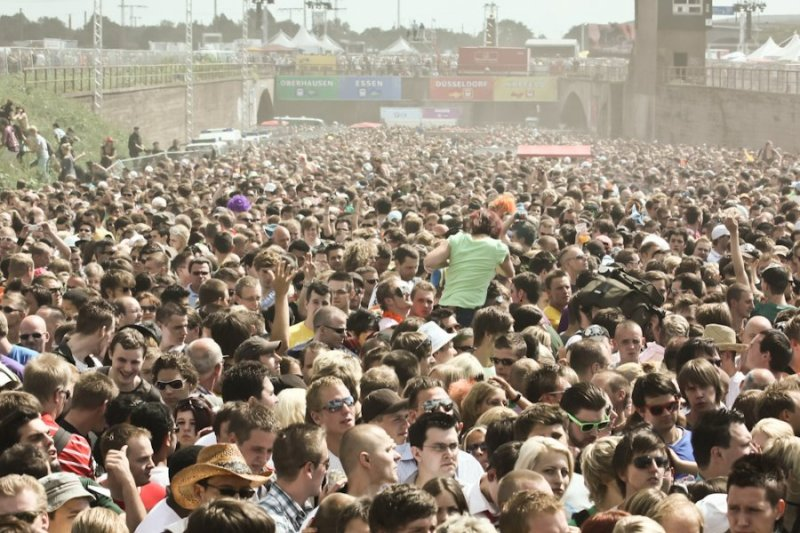
\includegraphics[width=.45\linewidth]{ac}}\\
\caption{(a) là hình ảnh trong cuộc hành hương ở Sabarimala và (b) là hình ảnh trong lễ hội âm nhạc Love Parade}	
\label{2figs}
\end{figure}

	Với những ứng dụng thiết thực và kể trên. Nhưng trong thực tế, cho đến nay việc giám sát đám đông qua các thiết bị thu phát hình ảnh vẫn chủ yếu dựa vào con người. Tuy nhiên, việc duy trì sự tập trung của con người cho việc giám sát một cách liên tục dễ gây quá tải cho người giám sát dẫn đến những sai sót có thể xảy ra, bên cạnh đó công việc này còn đòi hỏi chi phí vận hành, quản lý cao và khó giám sát. Từ đó, việc xây dựng các hệ thống phát hiện và ước lượng đám đông hay phương tiện giao thông là một nhu cầu cấp thiết hiện nay. Hệ thống này có thể hỗ trợ con người giám sát hiệu quả những hoạt động có liên quan đến tụ tập đám đông hay những điểm nóng giao thông đang gây ùn tắc, để từ đó đưa ra những cảnh báo hay chiến lược giải quyết phù hợp và hiệu quả. \par 
	Với tính ứng dụng cao và thiết thực, nhưng đổi lại đây là một bài toán vẫn còn tồn tại rất nhiều thách thức và khó khăn cần phải giải quyết và cải thiện như: sự che khuất lẫn nhau giữa các đối tượng, kích thước đa dạng của các đối tượng (tùy thuộc vào độ sâu của ảnh), sự biến dạng đối tượng từ góc nhìn, quá ít pixel để biểu diễn cho đối tượng... vv. Qua quá trình tìm hiểu và khảo sát cho bài toán đếm đối tượng, sinh viên nhận thấy hướng tiếp cận giải quyết bài toán theo phương pháp regression đã cho kết quả với tốc độ và độ chính xác cao nhất hiện nay. Kèm theo đó, Deep Learning trong thời gian gần đây đã phát triển rất nhanh chóng và được áp dụng hiệu quả trong nhiều lĩnh vưc. Đặc biệt là về Computer Vision, Deep Learning đã giải quyết rất tốt với độ chính xác cao các vấn đề trong lĩnh vực này (bài toán phân lớp ảnh áp dụng deep learning cho độ chính xác thậm chí còn tốt hơn con người). Chính vì những lý do trên, sinh viên chọn thực hiện khóa luận này với đề tài "nghiên cứu ứng dụng deep learning vào bài toán đếm đối tượng trong ảnh tĩnh".  
\section{Đối tượng, pham vi và mục tiêu} 
\subsection{Đối tượng}
Đối tượng nghiên cứu là các phương pháp áp dụng deep learning để ước lượng mật độ đám đông (con người hoặc phương tiện giao thông) trong các hình ảnh tĩnh. 
\subsection{Phạm vi}
\begin{itemize}
\item Khóa luận tập trung tìm hiểu Deep Learning mà cụ thể là mô hình Convolutional Neural Networks qua đó áp dụng để giải quyết bài toán đếm đối tượng.
\item Thực hiện huấn luyện và đánh giá trên ba bộ dữ liệu:
	\begin{itemize}
 	\item TRANCOS\footnote{http://agamenon.tsc.uah.es/Personales/rlopez/data/trancos/} bộ dữ liệu được thu thập từ các video giám sát giao thông ở thành phố Dirección General de Tráfico Tây Ba Nha\footnote{http://www.dgt.es/es/}.
	\item UCSD\footnote{http://www.svcl.ucsd.edu/projects/peoplecnt/} bộ dữ liệu này thu thập từ dữ liệu video được lấy từ camera giám sát, chưa cảnh người đi bộ trên một con đường ở UCSD (University of California, San Diego\footnote{https://ucsd.edu/}).
	
	\item UCF\footnote{$http://crcv.ucf.edu/data/crowd_counting.php$} là bộ dữ liệu chứa các hình ảnh đám đông với mật đố cực lớn. Các hình ảnh này được thu thập từ FLICKR\footnote{là một trang web lưu trử dữ liêu hình ảnh và video được xây dựng bởi Ludicorp trong năm 2004 và sau đó Yahoo mua lại vào 20 tháng 3 năm 2015}. 
	\end{itemize}
\item xây dựng ứng dụng đánh giá kết quả thực nghiệm và ướng lượng đối tượng (người và phương tiện giao thông) trong ảnh tĩnh.
\end{itemize}

\subsection{Mục tiêu}
\begin{itemize}
\item	Tập trung tìm hiểu về Deep Learning và mô hình Convolutional Neural Networks.
\item 	Khảo sát về bài toán đếm đối tượng, các chiến lược được để xuất giải quyết bài toán, tìm hiểu các kiến thức liên quan. Từ đó chọn chiến lược hiệu quả nhất để áp dụng và giải quyết bài toán đếm đối tượng. 
\item 	So sánh đánh giá giải pháp xây dựng được với những công trình đã được công bố.
\item	Xây dựng công cụ đáng gía mô hình và ứng dụng ước lượng đám đông và phương tiện giao thông.

\end{itemize}

\section{Cấu trúc khóa luận}
\textbf{Chương 1: } Giới thiệu tổng quan đề tài.
\\\textbf{Chương 2: } Trình bày tổng quát các hướng tiếp cận đã được đề xuất nhằm giải quyết bài toán hướng đối tượng đã được đưa ra. 
\\\textbf{Chương 3: } Trình bày các kiến thức cơ sở về Neural Networks, Deep Learning, Convolutional Neural Network và từ đó trình bày mô hình Deep Learning áp dụng cho bài toán.
\\\textbf{Chương 4: } Trình bày phương pháp đánh giá mô hình trên các bộ dữ liệu và đưa ra so sánh với các phương pháp khác. kèm theo đó trình bày ứng dụng xây dựng công cụ đánh giá và áp dụng mô hình để ước lượng đối tượng. 
\\\textbf{Chương 5: } Trình bày ứng dụng thực nghiệm, kết luận và hướng phát triển của đề tài.



